\documentclass{llncs}
\usepackage{graphicx}
\usepackage{charter} 

\newcommand{\E}{\mathbf{E}\,}

\newcommand{\dlom}{\textsc{dl-om}}
\newcommand{\DLOM}{DL-OM}
\date{}
\begin{document}
\title{Approximate Range Mode and Range Median Queries
\thanks{This work is supported in part by NSERC (Natural Sciences and 
Engineering Research Council of Canada) and MITACS (Mathematics of Information 
Technology and Complex Systems) grants.}}

\author{Prosenjit Bose \and 
Evangelos Kranakis\and 
Pat Morin\and 
Yihui Tang}

\institute{School of Computer Science, Carleton University \\
Ottawa, Ontario, K1S 5B6, Canada\\
\email{\{jit,kranakis,morin,y\_tang\}@scs.carleton.ca} }

\maketitle

\begin{abstract}
We consider data structures and algorithms for preprocessing a labelled 
list of length $n$ so that, for any given indices $i$ and $j$ we can answer 
queries of the form: What is the mode or median label in the sequence 
of labels between indices $i$ and $j$. Our results are on approximate 
versions of this problem. Using $O(\frac{n}{1-\alpha})$ space, our data 
structure can find in $O(\log\log_{\frac{1}{\alpha}}n)$ time an 
element whose number of occurrences is at least $\alpha$ times 
that of the mode, for some user-specified parameter $0<\alpha<1$. 
Data structures are proposed to achieve constant query time 
for $\alpha = 1/2, 1/3 \mbox{ and } 1/4$, using storage space of
$O(n\log n), O(n\log\log n)$ and $O(n)$, respectively.
Finally, if the elements are comparable, we construct an
$O(\frac{n}{1-\alpha})$ space data structure that answers approximate range
median queries. Specifically, given indices $i$ and $j$, in $O(1)$
time, an element whose rank is at least $\alpha \times \lfloor
|j-i+1|/2\rfloor$ and at most $(2-\alpha) \times \lfloor
|j-i+1|/2\rfloor$ is returned for $0 <\alpha<1$.
\end{abstract}

\section{Introduction}
Let $A= a_1,\ldots,a_n$ be a list of elements of some data type. 
We wish to construct data structures on $A$, such that we can 
quickly answer {\it range queries}. These queries take two indices 
$i$, $j$ with $1 \leq i \leq j \leq n$ and require computing 
$F(a_i,\ldots,a_j)=a_i \circ a_{i+1} \circ \cdots \circ a_{j-1} \circ
a_{j}$. If the inverse of the operation ``$\circ$'' exists, 
then range queries have a trivial solution of linear space and 
constant query time. For example, if ``$\circ$'' is arithmetic
addition (subtraction being its inverse), we precompute all the partial 
sums $b_i = a_1 + \cdots +a_i, i=1,\ldots,n$, and the range query 
$F(a_i,\ldots,a_j)=a_i + \cdots + a_j$ can be answered in constant 
time by computing $b_j - b_{i-1}$. Yao \cite{yao82} 
(see also Alon and Schieber \cite{as87}) showed that if 
``$\circ$'' is a constant time semigroup operation (such as
maximum or minimum) for which 
no inverse operation is allowed, and $a \circ b$ can be computed 
in constant time then it is possible to answer range queries in 
$O(\lambda(k,n))$ time using a data structure of $O(kn)$ size, 
for any integer $k \ge 1$. Here $\lambda(k,\cdot)$ is a slowly 
growing function at the $\lfloor k/2 \rfloor$-th level of the 
primitive recursive hierarchy. For example, 
$\lambda(2,n) = O(\log n)$, $\lambda(3,n) =
O(\log \log n)$ and $\lambda(4,n) = O(\log^* n)$.


Krizanc {\it et al} \cite{kms03} studied the storage space 
versus query time tradeoffs for range mode and range median queries. 
These occur when $F$ is the function that returns the mode or 
median of its input. Mode and median are two of the most 
important statistics \cite{am04,bccch00,llxy04,mrl98}. 
Given a set of $n$ elements, a {\it mode} 
is an element that occurs at least as frequently as any other 
element of the set. If the elements are comparable (for example, 
real numbers), the {\it rank} of an element is its position in 
the sorted order of the input. For example, the rank of the minimum 
element is 1, and that of the maximum element is $n$. The $\phi$-quantile 
is the element with rank $\lfloor \phi n \rfloor$. The $1/2$-quantile
is also called the {\it median}. Note the trivial solution 
does not work for  range mode or range median queries 
as no inverse exists for either operation.
Yao's approach does not apply either because neither range mode nor
range median is associative and therefore not a semigroup query. 
Also, given two sets $S_1$ 
and $S_2$ and their modes (or medians), the mode (or median) of the union 
$S_1 \bigcup S_2$ cannot be computed in constant time. New data structures are needed for
range mode and range median queries. 
Krizanc {\it et al} \cite{kms03} gave a data structure of 
size $O(n^{2-2\epsilon})$ 
that can answer range mode queries in $O(n^\epsilon \log n)$ time, where 
$0 < \epsilon \leq 1/2$ is a constant representing storage space-query
 time tradeoff.
For range median queries, they show that a data 
structure of size $O(n)$ can answer range median queries in
$O(n^\epsilon)$ time and a faster $O(\log n)$ query time can be achieved 
using $O(\frac{n\log^2n}{\log\log n})$ space.

    
In this paper we consider the approximate versions of range mode 
and range median queries. We show that if a small error is tolerable, 
range mode and range median queries can be answered 
much more efficiently in terms of storage space and query time.
Given a sublist $S=a_i,a_{i+1},\ldots,a_j$, an element is said to 
be an {\it approximate mode} of $S$ if its number of occurrences 
is at least $\alpha$ times that of the actual mode of {\it S}, 
where $0 < \alpha < 1$ is a user-specified  approximation factor.
If the elements are comparable, the {\it median} is the 
element with rank (relative to the sublist) 
$\lfloor (j-i+1)/2 \rfloor$.
An {\it $\alpha$-approximate median} of {\it S} is an element whose rank is
between $\alpha \times \lfloor (j-i+1)/2 \rfloor$ and 
$(2 - \alpha) \times \lfloor (j-i+1)/2\rfloor$. Clearly, there could be
several approximate modes and medians.

We show that approximate range mode queries can be answered in
\linebreak[4]$O(\log\log_{\frac{1}{\alpha}} n)$ time using a data 
structure of size $O(n)$. We also show that constant query 
time can be achieved for
$\alpha = 1/2, 1/3$ and $1/4$ using storage space of size $O(n\log n)$,
$O(n\log \log n)$ and $O(n)$, respectively. We introduce a constant 
query time data structure for answering approximate range median
queries. We also study the preprocessing time required for
the construction of these data structures.


To the best of our knowledge, there is no previous work
on approximate range mode or median queries. Two problems related 
to range mode and range median queries are {\it frequent elements}
and {\it quantile summaries} over sliding windows \cite{am04,llxy04}. 
For many applications, data takes the form of continuous 
data streams, as opposed to finite stored data sets.
Examples of such applications include
network monitoring and traffic measurements, financial transaction 
logs and phonecall records. All these applications view recently arrived 
data as more important than those a long time back. This preference 
for recent data is referred to as the {\it sliding window} 
model \cite{dgim02} in which the queries are answered regarding only 
the most recently observed $n$ data elements. Lin {\it et al}
\cite{llxy04} studied the problem of continuously maintaining 
quantile summaries over sliding windows. They devised an algorithm 
for approximate quantiles with an error of at most $\epsilon n$ using 
$O(\frac{\log \epsilon^2 n}{\epsilon} + \frac{1}{\epsilon^2})$ 
space in the worst case for a fixed window size $n$. For 
 windows of variable size at most $n$ (such as timestamp-based 
windows in which the exact number of arriving elements 
cannot be predetermined), $O(\frac{\log^2 \epsilon n}{\epsilon^2})$ 
storage space is required.
Arasu and Manku \cite{am04} improved both bounds to 
$O(\frac{1}{\epsilon}\log \frac{1}{\epsilon}\log n)$ and
$O(\frac{1}{\epsilon}\log \frac{1}{\epsilon} \log \epsilon n\log n)$
respectively. They also proposed deterministic 
algorithms for the problem of finding all
frequent elements ({\it i.e.,} elements with a minimum 
frequency of $\epsilon n$) using $O(\frac{1}{\epsilon} 
\log^2 \frac{1}{\epsilon})$
and $O(\frac{1}{\epsilon}\log^2 \frac{1}{\epsilon} \log \epsilon n)$
worst case space for fixed- and variable-size windows, respectively.  



 
\section{Approximate Range Mode Queries} 
Given a list of elements $a_1,\ldots,a_n$ and an approximation factor 
$0 < \alpha < 1$, the {\it  approximate range mode queries} can be specified 
formally as follows.\\
{\bf INPUT:} Two indices $i,j$ with $1 \leq i \leq j \leq n$.\\
{\bf OUTPUT:} An element $x$ in $a_i,\ldots,a_j$ such that 
$F_{x}(a_i,\ldots,a_j) \ge \alpha \times F(a_i,\ldots,a_j)$, where 
$F_{x}(a_i,\ldots,a_j)$ is the frequency\footnote{We use frequency 
and the number of
occurrences interchangeably throughout the paper.} of $x$ in 
$a_i,\ldots,a_j$ and $F{(a_i,\ldots,a_j)} =
\max_x{F_{x}(a_i,\ldots,a_j)}$ 
is the number of occurrences of a mode in $a_i,\ldots,a_j$.


Our data structure is based on the observation that given a fixed left end $i$ of a
query range, as the right end $j$ of the range increases, the number of times the
approximate mode changes as  $j$ varies 
from $i$ to $n$ is at most $\log_{\frac{1}{\alpha}} (n-i)$. 
This is because the same element can be output as approximate 
mode as long as no other element's
frequency exceeds $1/\alpha$ times that of the current approximate mode.
When the actual mode's frequency has exceeded $1/\alpha$ times that of the 
approximate mode, the approximate mode is replaced and the
actual mode becomes the new approximate mode.

For example, given the list of 20 elements shown in 
Figure~\ref{originalarray} and 
approximation factor $\alpha = 1/2$, $b$ is an approximate 
mode of $a_1,\ldots,a_{9}$ 
because $b$ occurs 2 times in the sublist, while 
the actual mode $a$ occurs 4 times in the same sublist. 
But this is no longer true for query $a_1,\ldots,a_{10}$, 
as the number of occurrences of $b$ is
still 2 while the actual mode $a$ occurs 5 times in the sublist
$(F_{a}(a_1,\ldots,a_{10})=5)$.  
In this case, either $a$ or $c$ $(F_{c}(a_1,\ldots,a_{10})=3)$ is a valid approximate mode. 

\begin{figure}[htb]\label{originalarray}
\centering
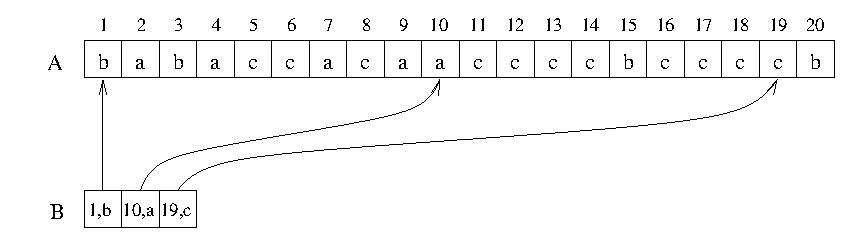
\includegraphics[width=4.8in]{oa}
\caption{$\alpha=1/2$. A lookup table of size 3 is used for answering queries
  $a_1,\ldots,a_j$, $j=1,\ldots,20.$ For example, $a$ is an approximate mode of
  $a_1,\ldots,a_{15}$ because $a$ occurs at
  least 5 times in the query range $(F_a(a_1,\ldots,a_{15})=5 )$
while no other element occurs more than 10 times until $j=19$ $(F_c(a_1,\ldots,a_{19})=11)$.} 
\label{originalarray}
\end{figure}

Assuming $a$ is chosen to be the new approximate mode, it remains a
valid approximate mode as the right end of the query range increases until 
$j=19$ at which point the actual mode $c$ occurs 11 times ($F_{c}(a_1,\ldots,a_{19})=11$). 
Since no other element ($a$ or $b$) occurs more than or equal to half of the actual mode 
($F_a(a_1,\ldots,a_{19})=5,F_b(a_1,\ldots,a_{19})=3$), $c$ is now the only 
approximate mode until $j=20$. Since an approximate
mode remains valid until another element occurs more than $1/\alpha$ times the
current approximate mode, the number of approximate modes that have to be stored is much 
less than the number of elements of the original list. As shown in the 
example of Figure~\ref{originalarray}, instead 
of storing the complete original array of 20 elements, a table of 3 approximate modes is used to 
answer all approximate range mode queries $a_1,\ldots,a_j,1 \leq j \leq 20$.  


Given an approximation factor $\alpha$, all approximate range mode queries 
with $a_1$ being the left end: 
$a_1,\ldots,a_j$ $(1\leq j \leq n)$ can be answered using $O(\log_{\frac{1}{\alpha}} n)$
storage space. The data structure is a lookup table $B=a_{c_1}$, $\ldots,a_{c_m}(1 \leq
c_1 < c_2 < \ldots < c_m \leq n)$ in which we store $m$ approximate modes. 
The first entry is always $a_1$ $(c_1 = 1)$. The second entry $a_{c_2}$
is the first element in $A$ that occurs $\lceil 1/\alpha \rceil$ times, 
{\it i.e.}, 
$F_{a_{c_2}}(a_1, \ldots, a_{c_2}) = \lceil 1/\alpha \rceil$ and 
$F_{a_{c_2}}(a_1, \ldots, a_{c_2}) > F_{a_i}(a_1,\ldots,a_{c_2})$
for $\forall i \neq c_2$. 
In general, the $k$th entry in the table is the first element in $A$ that 
occurs $\lceil 1/\alpha^{k-1} \rceil$ times in the sublist 
as the right end of the query range increases. 
Note that $a_{c_k}$ is an approximate mode of 
$a_1,\ldots,a_j$ for any $c_k\leq j < c_{k+1}$ since $a_{c_k}$ occurs at least
$\lceil 1/\alpha^{k-1} \rceil$ times in $a_1,\ldots,a_j$ 
$(F_{a_{c_k}}(a_1,\ldots,a_j) \ge F_{a_{c_k}}(a_1,\ldots,a_{c_k}) = 
\lceil 1/\alpha^{k-1} \rceil)$, 
while no other element occurs more than $1/\alpha^k$ times in the same range
$(F_x(a_1,\ldots,a_j) < F_{c_{k+1}}(a_1,\ldots,a_{c_{k+1}}) = \lceil 1/\alpha^k \rceil)$.

The last approximate mode in the table, $a_{c_m}$, occurs at least 
$\lceil 1/\alpha^{m-1} \rceil$ times in $a_1,\ldots,a_n$. It follows 
immediately that the number of approximate modes stored in the lookup table 
$m$ is at most $\log_{\frac{1}{\alpha}} n + 1$. 

To answer approximate range mode queries in the range
$a_1,\ldots,a_j$, binary search is used to
find in $O(\log\log_{\frac{1}{\alpha}} n)$ time the largest $c_k$ that is  
less than or equal to  $j$ and output $a_{c_k}$ as the answer.

\begin{lemma}\label{simple results}
There is a data structure of size $O(\log_{\frac{1}{\alpha}} n)$ that can answer
approximate range mode queries in the range $a_1,\ldots,a_j$ $(1 \leq j \leq n)$ in 
$O(\log\log_{\frac{1}{\alpha}} n)$ time.
\end{lemma}

An immediate application of Lemma~\ref{simple results} is a data 
structure for answering approximate range mode queries with 
arbitrary ends. The data structure is a collection of $n$ 
lookup tables $(T_i, i=1,\ldots,n)$, one table for each left end. 
An auxiliary array of $n$ pointers is used to locate a table 
in $O(1)$ time. A query $a_i, \ldots,a_j$ can be answered by 
first locating table $T_i$ in $O(1)$ time,  and 
then searching in $T_i$ to find the approximate 
mode of $a_i,\ldots,a_j$, which takes $O(\log\log_{\frac{1}{\alpha}} n)$ time 
since $T_i$ contains at most $O(\log_{\frac{1}{\alpha}} (n-i)) = O(\log_{\frac{1}{\alpha}} n)$ approximate modes.


\begin{corollary}
There is a data structure of size $O(n\log_{\frac{1}{\alpha}} n)$ that can answer approximate  range queries
in $O(\log\log_{\frac{1}{\alpha}} n)$ time. 
\end{corollary}


\subsection{An Improvement Based on Persistent Search Trees}


We have seen that by maintaining a lookup table $T_i$ of 
size $O(\log_{\frac{1}{\alpha}} n)$ 
for each left end $i$ $(1 \leq i \leq n)$ 
and using $O(n\log_{\frac{1}{\alpha}} n)$ total storage space, 
any approximate range mode query in the range
$a_i,\ldots,a_j$ can be answered in $O(\log\log_{\frac{1}{\alpha}} n)$ 
time. Given a fixed left end 
$i$, storing an answer for each right end $j$ is not necessary since 
the answer to the query changes less frequently as $j$ varies. 
The approximate modes of two query ranges with adjacent right ends are unlikely to be 
different. In this section, 
we pursue this idea and show that storage of a complete lookup table for each left end is not 
necessary because of the similarity between two tables with adjacent left ends.  

To see how the approximate range mode changes gradually as
the two ends of a query range move, we need a systematic way 
to keep track of the range within 
which the current approximate mode remains a valid approximation of 
the actual mode and its number of occurrences in that range. As the query range 
changes, the frequency of the current approximate mode may also
change. Once it drops below a predetermined threshold value
($f_{low}$, the calculation of which will be discussed next), 
a new approximate mode is chosen and the query range updated. 

As shown in Table~\ref{lookup table general form}, each entry in 
the lookup table is a 5-tuple $(f_{low_r},
f_{high_r},$ \linebreak[2] $q_r,$ 
\linebreak[2]$ans_r, f_{ans_r})$. 
Given an approximation factor $\alpha$, $[f_{low_r}, f_{high_r}]$ are precomputed 
for $r=1,\ldots,2\lceil \log_{\frac{1}{\alpha}} n \rceil$  and
remain the same for all tables.\\

\begin{table}[htb]
\begin{center}
{\tt
\begin{tabular}{|c|c|c|}\hline
Frequency Range & Query Range    & Answer \\\hline\hline  
\ldots & & \\\hline
$[f_{{low}_r}$, $f_{{high}_r}]$ & $q_r$  & $(ans_r,f_{{ans}_r})$ \\\hline
$[f_{{low}_{r+1}}$, $f_{{high}_{r+1}}]$ & $q_{r+1}$ & $(ans_{r+1},f_{{ans}_{r+1}})$ \\\hline
\ldots & &
\\\hline 
\end{tabular}
}\caption{\label{lookup table general form}
$f_{{low}_1}=1$, $f_{{high}_1}=1$, 
$f_{{low}_{r+1}} = f_{{high}_{r}} + 1$, 
$f_{{high}_{r+1}}=\lceil f_{low_{r}}/\alpha \rceil + 1$,
$F(a_i,\ldots,a_{q_r})=f_{{high}_r}$, $f_{{ans}_{r}}=F_{{ans}_r}(a_i,\ldots,a_{q_r})$, 
$f_{{low}_{r}} \leq f_{{ans}_{r}} \leq  f_{{high}_{r}}$.
}
\end{center}
\end{table}
As noted before, the $i$th table $T_i$ corresponds to all the range
queries with the same left end $i$. A counter is set for each
element to keep track of its frequency as the right 
end $j$ varies. Given the fixed left end $i$, as the right end $j$
proceeds, $ans_r$ is the first element whose frequency in
$a_i,\ldots,a_j$ reaches $f_{high_r}$, and $q_{r+1}$ is the 
rightmost point up to which $ans_r$ remains a valid approximate 
mode, {\it i.e.,} no other element has a frequency higher than
$f_{high_r}/\alpha$. 
Given a query $a_i,\ldots,a_j$ with $q_r \leq j < q_{r+1}$, 
$ans_r$ is a valid approximate mode since its frequency is at least $f_{high_r}$ while no other 
element has a frequency higher than or equal to $f_{high_{r+1}}-1 =
\lceil f_{low_r}/\alpha \rceil$. To see how the subsequent tables are built based
on $T_i$ with minimum number of changes, the right end of the query
range is fixed, as the left
end of the query range proceeds, $ans_r$'s frequency may decrease, but 
it remains a valid approximate mode as long as $f_{ans_r} \ge
f_{low_r}$ and it is copied to the next table along with a possibly
smaller $f_{ans_r}$ (Note that $f_{ans_r}$ is needed only for 
bookkeeping purposes). The only time that
 $ans_r$ must change for a table is when its frequency 
drops below $f_{low_r}$. At this point we update 
$ans_r$ and the new approximate mode is the first element 
whose frequency reaches $f_{high_r}$ with respect to the 
current left end of query range. 
The query range $q_r$ is also updated to reflect the change on the approximate mode 
($F_{ans_r}(a_i,\ldots,a_{q_r}) = f_{high_r}$).  


\begin{table}[htb]\label{table of 20}
\begin{center}
\begin{tabular}{|r|r|r|r|r|r|r|r|r|r|r|r|r|r|} \hline
$T_i$    &$T_1$                  &$T_2$                &$T_3$               &$T_4$              &$T_5$             \\
$a_i$    &b                      &a                    &b                   &a                   &c             \\ \hline 
$[1,1]$  &$1,({\bf b},1)$        &$2,({\bf a},1)$      &$3,({\bf b},1)$     &$4,({\bf a},1)$     &$5,({\bf c},1)$ \\ 
$[2,3]$  &$7,({\bf a},3)$        &$7,(a,3)$            &$7,(a,2)$           &$7,(a,2)$           &$8,({\bf c},3)$\\
$[4,5]$  &$10,({\bf a},5)$       &$10,(a,5)$           &$10,(a,4)$          &$10,(a,4)$          &$12,({\bf c},5)$\\
$[6,9]$  &$17,({\bf c},9)$       &$17,(c,9)$           &$17,(c,9)$          &$17,(c,9)$          &$17,(c,9)$  \\ 
$[10,13]$&$20,({\bf c},11)$      &$20,(c,11)$          &$20,(c,11)$         &$20,(c,11)$         &$20,(c,11)$  \\ \hline    
\multicolumn{6}{c}{}\\ \hline
$T_i$     &$T_6$                 &$T_7$                   & $T_8$                 & $T_9$                 &$T_{10}$ \\
$a_i$     &c                   & a                    & c                   & a                   &a  \\ \hline
$[1,1]$   &$6,({\bf c},1)$     &$7,({\bf a},1)$       &$8,({\bf c},1)$      &$9,({\bf a},1)$      &$10,({\bf a},1)$\\
$[2,3]$   &$8,(c,2)$           &$10,({\bf a},3)$      &$10,(a,2)$           &$10,(a,2)$           &$13,({\bf c},3)$\\
$[4,5]$   &$12,(c,4)$          &$14,({\bf c},5)$      &$14,(c,5)$           &$14,(c,4)$           &$14,(c,4)$ \\
$[6,9]$   &$17,(c,8)$          &$17,(c,7)$            &$17,(c,7)$           &$17,(c,6)$           &$17,(c,6)$  \\ 
$[10,13]$ &$20,(c,10)$         &{\bf ---}             &---                  &---                  &--- \\ \hline    
\multicolumn{6}{c}{}\\ \hline
$T_i$    &$T_{11}$                &$T_{12}$                &$T_{13}$                &$T_{14}$                &$T_{15}$ \\ 
$a_i$    &c                     &c                     &c                     &c                     & b \\ \hline 
$[1,1]$  &$11,({\bf c},1)$      &$12,({\bf c},1)$      &$13,({\bf c},1)$      &$14,({\bf c},1)$      &$15,({\bf b},1)$ \\
$[2,3]$  &$13,({\bf c},3)$      &$13,(c,2)$            &$16,({\bf c},3)$      &$16,(c,2)$            &$18,({\bf c},3)$ \\
$[4,5]$  &$14,(c,4)$            &$17,({\bf c},5)$      &$17,(c,4)$            &$19,({\bf c},5)$      &$19,(c,4)$  \\
$[6,9]$  &$17,(c,6)$            &$19,({\bf c},7)$      &$19,(c,6)$            &{\bf ---}             & --- \\  
$[10,13]$&---                   &---                   &---                   &---                   &---\\ \hline    
\multicolumn{6}{c}{}\\ \hline
$T_i$    &$T_{16}$                &$T_{17}$                &$T_{18}$                &$T_{19}$              &$T_{20}$ \\
$a_i$    & c                    & c                    & c                    & c                    & b \\ \hline
$[1,1]$  &$16,({\bf c},1)$      &$17,({\bf c},1)$      &$18,({\bf c},1)$      &$19,({\bf c},1)$      &$20,({\bf b},1)$\\
$[2,3]$  &$18,(c,3)$            &$18,(c,2)$            &$19,({\bf c},2)$      &{\bf ---}             & --- \\
$[4,5]$  &$19,(c,4)$            &{\bf ---}             & ---                  & ---                  & --- \\
$[6,9]$  & ---                  & ---                  & ---                  & ---                  & --- \\ 
$[10,13]$&---                   &---                   & ---                  & ---                  & --- \\ \hline   

\end{tabular}\caption{\label{a lookup table example}An example showing the data structure for
answering $1/2$-approximate range mode queries on a list of 20 elements. Updates are in bold.}

\end{center}
\end{table}

Table~\ref{a lookup table example} shows the data structure for answering
approximate range mode queries on the same list as in Figure~\ref{originalarray}. 
For example, to look up the approximate mode of $a_4, \ldots, a_{12}$, we search 
in $T_4$ and find the entry with the largest $q_r$ that is smaller than 12: 
$\{[4,5],10,(a,4)\}$. This tells us that, in the sequence of $a_4,
\ldots, a_{12}$, $a$ occurs at 
least 4 times ($F_a(a_4,\ldots,a_{12}) \ge F_a(a_4,\ldots,a_{10}) = 4$) 
and no element occurs more than $8$ times ($F_x(a_2,\ldots,a_{12}) \leq F(a_2,\ldots,a_{17}) -1 = 8$).

After $T_1$ is built,  $T_i$ $(i\ge 2)$ is built based on $T_{i-1}$
with necessary updates. The number of updates made is given by the 
following lemma.

\begin{lemma}
\label{number of changes}
If the $r$th row of the table is updated in $T_{i}$, then it does not need to be updated 
in $T_{k}$ for any $i<k<i+1/\alpha^{\lfloor r/2 \rfloor}$.
\end{lemma}
\begin{proof}
When the $r$th row is updated in $T_{i}$, we set $ans_r$ to be the first element such that 
$F_{ans_r}(a_i, \ldots, a_{q_r}) = f_{high_r}$. Its frequency $f_{ans_r}$ is initially $f_{high_r}$ in $T_{i}$. 
Although $f_{ans_r}$ may decrease as $i$ increases, $ans_r$ does not need to be 
updated again until $f_{ans_r}$ drops below $f_{low_r}$, which takes at least 
$f_{high_r} - (f_{low_r} - 1) = f_{high_r} - f_{high_{r-1}} = 1/\alpha^{\lfloor r/2 \rfloor}$ 
steps.
\end{proof}

Note that there are no more than $2\lceil \log_{\frac{1}{\alpha}} n \rceil$ rows in a table and every time we 
build a new table, the first row needs to be updated. Lemma~\ref{number of changes} 
shows that the $r$th $(r \ge 2)$ row changes no more than $\alpha^{\lfloor r/2 \rfloor} n$ times 
during the construction of all $n$ tables.  
The total number of updates we have to make 
is given by the following theorem.

\begin{theorem}\label{number of updates in mode query}
The total number of updates we have to make is $O(n/(1-\alpha))$.
\end{theorem}
\begin{proof} $\mbox{Total number of updates} \leq n + 
\sum_{r=2}^{2 \lceil \log_{\frac{1}{\alpha}} n\rceil}{\alpha^{\lfloor r/2 \rfloor} n}
                                 =   O(\frac{n}{1-\alpha})$.
\end{proof}

Theorem~\ref{number of updates in mode query} says that, the majority of the table entries
can be reconstructed by referring to other tables. In other words,
although $n$ lookup tables are needed to answer approximate range mode queries, many of them
share common entries. A persistent search tree~\cite{dsst89} is used to store the tables 
efficiently. It has the property that 
the query time is $O(\log m)$ where $m$ is the number of entries in each table, 
and the storage space is $O(1)$ per update. In the case of approximate range mode 
queries, although each table can have as many as
$2\lceil\log_{\frac{1}{\alpha}} n \rceil$ entries, many tables share
the same entries and the number of different nodes in the persistent tree 
is $O(n/(1-\alpha))$, one for each update, and the query 
time for a node is $O(\log\log_{\frac{1}{\alpha}}{n})$. 

To build the search tree, we need to keep track of the 
frequency of each element as query range varies. 
The idea presented in~\cite{dlm02} leads to an algorithm that
maintains a counter for each element and the total preprocessing time
is $O(n\log_{\frac{1}{\alpha}} n +n\log n)$.

\begin{theorem}\label{mode}
There exists a data structure of size $O(n/(1-\alpha))$ that can answer approximate 
range mode queries in $O(\log\log_{\frac{1}{\alpha}} n)$ time, and can be constructed 
in $O(n\log_{\frac{1}{\alpha}} n +n\log n)$ time.
\end{theorem}



\subsection{Lower Bounds}


Next we show there is no faster worst case algorithm to 
compute the approximate mode for any fixed approximation factor
$\alpha$. 
To see this, let $A$ be a list of $n/\lceil 1/\alpha \rceil$ 
elements and $B=A \ldots A=b_1, \ldots, b_n$ is a list of length $n$ 
obtained by repeating $A$ $\lceil 1/\alpha \rceil$ times. 
The problem of testing whether there exist two identical elements in $A$ 
(also called {\it element uniqueness}) can be reduced to asking if the mode 
of $B$ occurs more than $\lceil 1/\alpha \rceil$ times. In the case of 
approximate range mode query, the answer to query $b_1,\ldots, b_n$ is 
an element whose frequency is greater than 1 if and only if the actual 
mode of $B$ occurs more than $\lceil 1/\alpha \rceil$ times. 

In the algebraic decision tree model of computation, the running time of 
determining whether all the elements of $A$ are unique is known to have 
a complexity of $\Omega(n \log n)$ \cite{o83}. However, 
this problem can also be 
solved by doing a single approximate range mode query $b_1,\ldots, b_n$ 
after preprocessing $B$, which implies the same lower bound holds for 
approximate range mode queries.

\begin{theorem}
Let $P(n)$ and $Q(n)$ be the preprocessing and query times, respectively, 
of a data structure for answering approximate mode queries, we have 
$P(n) + Q(n) = \Omega(n\log n)$.
\end{theorem}

On the other hand, $\Omega(n)$ storage space is required by any data structure
that supports approximate range mode queries since the original list can be 
reconstructed by doing queries $(a_1,a_1),(a_2,a_2),\ldots,(a_n,a_n)$, 
regardless of what value $\alpha$ is.


\subsection{Constant Query Time}
Yao \cite{yao82} (see also Alon {\it et al} \cite{as87}) showed that if
a query $a_i, \ldots, a_j$ 
can be answered by combining answers of queries $a_i, \ldots, a_x$ and 
$a_{x + 1}, \ldots, a_j$ in constant time, then
$\Theta(n\lambda(k,n))$ time and space is both necessary and sufficient 
to answer range queries in at most $k$ steps. We adapt the same
approach to develop constant query time data structures for some
special cases of approximate range mode queries. Namely, the
approximation factor $\alpha = 1/k$ where $k$ is some positive integer.

The following lemma says that, if we can partition the range 
$a_i,\ldots,a_j$ into $k$ intervals and we know the mode of each 
interval, then one of these is an approximate mode, for $\alpha = 1/k$.

\begin{lemma}\label{k intervals}If $\{B_1,\ldots,B_k\}$ is a partition 
of $a_i,\ldots,a_j$ then $max_pF(B_p) \geq$ \linebreak[4] $F(a_i, \ldots, a_j)/k$.
\end{lemma}
\begin{proof}
By contradiction. Otherwise for any element $x$ we have 
$F_x(a_i,\ldots,a_j) = \sum_{p=1}^{k}F_x(B_p) 
\leq k \times max_pF(B_p) <  F(a_i, \ldots, a_j)$.
\end{proof}

Yao \cite{yao82} and Alon {\it et al} \cite{as87} gave an optimal 
scheme of using a minimum set of intervals  
such that any range $a_i,\ldots,a_j$ can be covered by at most $k$ such intervals. 

\begin{lemma}\label{alon}(Yao \cite{yao82}, Alon {\it et al} \cite{as87})
  There exists a set of
 $O(n\lambda(k,n))$ intervals such that
any query range $a_i, \ldots, a_j$ can be partitioned into at 
most $k$ of these intervals. Furthermore, given $i$ and $j$, 
these intervals can be found in $O(k)$ time.
\end{lemma}

Given Lemma~\ref{k intervals} and Lemma~\ref{alon}, we 
immediately obtain a constant query time solution to 
approximate range mode queries with approximation factor $1/k$.
By precomputing the mode of each interval, a query can be answered 
by first fetching the partition of the 
query range, which is a set of at most $k$ intervals, and then 
outputting the one with the highest frequency among $k$ modes of these intervals.  

\begin{theorem}\label{1/2 and 1/3}There exists a data structure of
  size $O(n\lambda(k,n))$ 
that can answer approximate 
range mode in $O(k)$ time, for $\alpha=1/k$.
\end{theorem}

The results in Theorem~\ref{1/2 and 1/3} can be further 
improved using a table lookup trick for $k \ge 4$. 
We partition the list into $n/\log n$ blocks of size 
$\log n$, $B_i=a_{(i-1)\log n +1},\ldots,a_{i\log n}, 
i =1, \ldots, n/\log n$. By Lemma~\ref{alon}, there exists 
a set of $O((n/\log n)\lambda(2,n/\log n))=O(n)$ 
intervals such that any range with both ends at the 
boundaries of the blocks can be covered with at most 
2 of these intervals. The exact modes of these intervals are
precomputed. Inside every block, exact modes of 2 
intervals are precomputed for each element, one interval is 
between the element and the beginning of
the block and the other interval between the element and the 
end of the block.
Any query range that spans more than one block can be partitioned 
into at most 4 intervals. The first one is the (possibly partial) 
block in which the range starts; the last one is the
the (possibly partial) block in which the range ends and the other 
(at most) two intervals in between 
cover all the remaining blocks (if any).  Of these intervals the 
modes are all precomputed, and the 
one with the highest frequency is a $1/4$-approximation of the 
actual mode. 

It remains to show that a query within a block can also be 
answered in $O(1)$ time. 
This is done by recursively partitioning the $\log n $ block 
into $\log n / \log\log n$ blocks of size 
$\log\log n$. The same method above is used to preprocess 
these blocks, and the result 
is a data structure of $O(n)$ size that can answer any query 
that spans more than one 
$\log\log n$-block in $O(1)$ time. 

To answer queries within a $\log\log n$-block, a standard data
structure trick \cite{gt85} of canonical subproblems is used. 
Note that we can normalize each block by replacing each 
element with
the index of its first occurrence within the block. Because 
such index
is a non-negative integer that is at most $\log\log n$ and each 
block consists of $\log\log n$ such
values, there are at most $(\log\log n) ^{\log\log n}$ different 
blocks. Among all
$n/\log\log n$ blocks of size $\log\log n$, many are of the 
same type. Thus, preprocessing of each block is unnecessary, and 
storage space 
can be reduced by preprocessing a block once and reusing the results for all blocks of 
the same type. The data structure used is a
$\log\log n \times \log\log n$ matrix that can answer range mode query in constant time.  
All the queries in blocks of the same type are done in the same matrix. There are at 
most $(\log\log n) ^{\log\log n}$ possible matrices which require $O((\log\log n) ^{\log\log n}(\log\log n)^2)=o(n)$ storage space.  
 

\begin{theorem}
There exists a data structure of size $O(n)$ that can answer approximate range mode
queries in $O(1)$ time, for $\alpha=1/4$.
\end{theorem}


\section{Approximate Range Median Queries}


In this section, we consider approximate range median queries on a list of comparable 
elements $A=a_1,\ldots,a_n$. Given an approximation factor $0 < \alpha < 1$, our 
task is to preprocess $A$ so that, given indices $1 \leq i \leq j \leq n$, we can 
quickly return an element of $a_i,\ldots,a_j$ whose rank is between
$\alpha \times \lfloor (j-i+1)/2 \rfloor$ and
$(2-\alpha) \times \lfloor (j-i+1)/2 \rfloor$.


To simplify the presentation we assume $n=2^d$ for some integer $d
\geq 1$. Generalization to arbitrary $n$ is straightforward. 
As shown in Figure \ref{median}, $d$ levels of partitions are used. In 
level $i$, the list is partitioned into $2^i$ non-overlapping blocks of 
size $n/2^i$. Exact medians of sublists with both ends at the boundaries
of the blocks (up to $2 \lceil 2 \alpha / (1- \alpha) \rceil$ blocks 
away) are precomputed. The idea behind 
our algorithm is that, if a query $a_i, \ldots, a_j$ spans many blocks, 
then the contribution of the first and last block is minimal and can
be ignored. Instead, we could simply answer the (precomputed) median 
of the union of the internal blocks. 
On the other hand, since we are using many different block sizes, we
can choose a partition level so that $a_i, \ldots, a_j$ spans just 
enough blocks for the strategy above to give a valid approximation. 
This ensures that we do not have to precompute too many medians.


At the lowest level, $a_1,\ldots,a_n$ is 
partitioned into $n$ blocks each consisting of a single element.
We precompute for each $i=1,\ldots,n$ all the medians of
$a_i,\ldots,a_j$, for $i \leq j \leq i+2 \lceil 2 \alpha / (1- \alpha)
\rceil -1$. This enables us to answer queries
of length no more than $2 \lceil 2 \alpha / (1- \alpha) \rceil$ in
$O(1)$ time using $O(n/(1-\alpha))$ space. To answer queries 
of length greater than 
$\lceil 2 \alpha / (1- \alpha)\rceil -1$, we search in a higher level 
where the query spans at least  $\lceil 2 \alpha / (1- \alpha) \rceil$ but no 
more than $2 \lceil 2 \alpha / (1- \alpha) \rceil$ complete blocks.
Suppose the query 
spans $\lceil 2 \alpha / (1- \alpha) \rceil 
\le c \le 2 \lceil 2 \alpha / (1- \alpha) \rceil$ complete blocks in level
$i$, let $l$ denote the length of the query, we have  
$cn/2^i \le l < (c+2) n/2^i$. The median of the union 
of these $c$ blocks is precomputed and
its rank in the query range is at least $cn/2^{i+1} \ge \alpha l/2 $ and at 
most $cn/2^{i+1} + (l-cn/2^i) \le (2-\alpha)l/2$, in other words,
it is an $\alpha$-approximate median of the query range.

  

\begin{figure}[htb]\label{median}
\centering
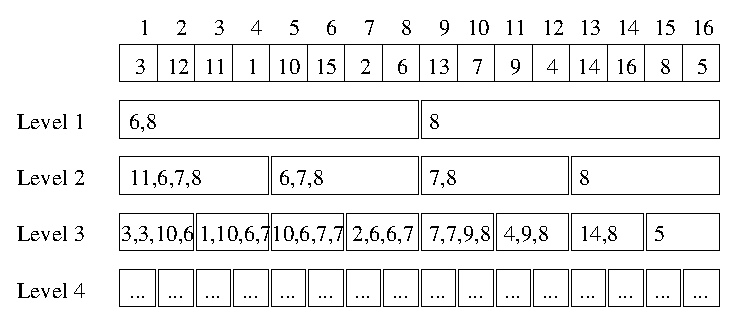
\includegraphics[height=4.5cm]{median}
\caption{$\alpha=1/2$. For each block up to $2 \lceil 2 \alpha /
  (1-\alpha) \rceil = 4$ medians
are precomputed. For example, associated with
the $2nd$ block in level 3 are 4 medians, each 
corresponds to a union of up to 4 consecutive 
blocks: $1=Median(B_{3_2})$;
$10=Median(B_{3_2} \bigcup B_{3_3})$; 
$6=Median(B_{3_2} \bigcup \ldots \bigcup B_{3_4})$;
$7=Median(B_{3_2} \bigcup \ldots \bigcup B_{3_5})$.  
Note that a 1/2-approximate range median query that spans more than 
4 complete blocks also spans
at least 2 complete blocks in the next higher level and therefore
can be answered in a higher level with sufficient accuracy. Range 
median queries are answered by looking in the level where 
the query range spans just enough number of complete blocks. 
For example, query $a_2,\ldots,a_{11}$ spans 4 complete level 3 
blocks ($B_{3_2}\bigcup \ldots \bigcup B_{3_5}$) but only 
1 complete level 2 block ($B_{2_2}$). Therefore, the $4th$ entry in 
the $2nd$ level 3 block ($T_{3_2}(4)=
{\mbox Median}(B_{3_2} \bigcup \ldots \bigcup B_{3_5}) = 7,
\mbox{whose rank in $a_2,\ldots,a_{11}$ is 4}$) is output as 
the approximate median, while the rank of the actual median 
is 5 in the sublist of 10 elements.}
\label{median}
\end{figure}




In the subsequent subsections we give the preprocessing time, 
storage space and query time of our data structure for
answering approximate range median queries.

\subsection{$O(n\log n/(1-\alpha)^2)$ Preprocessing Time}
We preprocess $A=a_1,\ldots,a_n$ and build $d$ lookup tables
as follows. To build $T_i$ $(1 \leq i \leq d)$, we partition $A$ 
into $2^i$ blocks each of size $n/2^i$:
$B_{i_j} = a_{(j-1) \times n/2^i + 1},$
\linebreak[3] $\ldots,$ \linebreak[3] $a_{j \times
  n/2^i}$, $j = 1, \ldots, 2^i$. $T_i$ has $2^i$ 
entries ($T_{i_j}, j = 1,2,\ldots,2^i$), each corresponds to a 
block $B_{i_j}$ and contains a pointer to a list of $2 \lceil
2 \alpha / (1-\alpha) \rceil$ elements of $A$:
$T_{i_j}(k) = Median(B_{i_j} \bigcup \ldots \bigcup B_{i_{j+k-1}} )$,
$k = 1, \ldots, 2 \lceil 2 \alpha / (1-\alpha) \rceil$.
$Median(B_{i_j} \bigcup \ldots \bigcup B_{i_{j+k-1}})$ is the 
median of $B_{i_j} \bigcup \ldots \bigcup B_{i_{j+k-1}}$,
which can be computed in $O(kn/2^i)$
time~\cite{bfprt73}. There are $\log n$ tables to be computed. It
follows that the total preprocessing time is $\sum_{i=1}^{\log
                                    n}\sum_{j=1}^{2^i}\sum_{k=1}^
                                  {2 \lceil \frac{2 \alpha}{1-\alpha}
                                    \rceil}
                                  O(\frac{kn}{2^i})
                                     =  O\left(\frac{n \log n}{(1-\alpha)^2}\right)$.



\subsection{$O(n/(1-\alpha))$ Storage Space}

The data structure for answering approximate range median 
queries is a set of $\log n$ lookup tables. Each table $T_i$ $(1 \leq i \leq \log n)$ 
has $O(2^i)$ entries and each entry is a list of at most $2\lceil
2\alpha / (1-\alpha)\rceil$ precomputed range medians, the 
total space needed to store all $\log n$ 
tables is $\sum_{i=1}^{\log n}{O(2^i \alpha/(1-\alpha))} =
O(n \alpha/(1-\alpha))=O(n/(1-\alpha))$. 


\subsection{$O(1)$ Query Time}
Next we show how to compute an approximate range median of
$a_i,\ldots,a_j$.
\begin{enumerate}
\item Compute the length of the query $l=j-i+1$, then locate table $T_p$ in which to 
continue the search: $p=\lceil \log\frac{2 \alpha n}{(1-\alpha)l} \rceil$.
\item Compute $b_i=\lceil \frac{i 2^p}{n} \rceil$ and $b_j=\lfloor
  \frac{j 2^p}{n} \rfloor$. Since 
$p=\lceil \log\frac{2 \alpha n}{(1-\alpha)l}\rceil < \log\frac{2
  \alpha n}{(1-\alpha)l}+ 1 = \log\frac{4 \alpha}{(1-\alpha)l}$, 
we have $2^p < \frac{4 \alpha n}{(1-\alpha)l}$ and
$b_j - b_i = \lfloor \frac{j 2^p}{n} \rfloor - \lceil \frac{i 2^p}{n}
 \rceil \leq \frac{(j-i)2^p}{n} \leq \frac{4(j-i)\alpha}{(1-\alpha)l}
 \leq \frac{4 \alpha}{1-\alpha} $. In other words, $Median(B_{p_{b_i}} 
\bigcup \ldots \bigcup B_{p_{b_j}}) $ 
is stored in a list to which a pointer is stored in $T_{p_{b_i}}$.
\item Output $T_{p_{b_i}}(b_j-b_i)=Median(B_{p_{b_i}} \bigcup \ldots
  \bigcup B_{p_{b_j}}) $ as the answer.
\end{enumerate}
Because each of the three steps above takes $O(1)$ time, the time required 
for answering the approximate range median query is $O(1)$. 

\begin{theorem}
There exists a data structure of size $O(n/(1- \alpha))$ that can
answer 
approximate range median queries
in $O(1)$ time, and can be built in $O(n\log n /(1-\alpha)^2)$ time.  
\end{theorem}


\bibliography{range}
\bibliographystyle{plain}


\end{document}
